% asset_id: FA22FlowsInNetworks2TikZ-003
\documentclass[tikz,border=8pt]{standalone}
\usepackage{amsmath}\usepackage{xcolor}\usetikzlibrary{arrows.meta,positioning,calc}
\definecolor{Canvas}{HTML}{FAF9F6}\definecolor{Panel}{HTML}{FFFFF0}\definecolor{LineSoft}{HTML}{E5E5EA}\definecolor{Ink}{HTML}{2C2C2E}\definecolor{Gold}{HTML}{C5A059}\definecolor{SoftRose}{HTML}{FBEFEF}\definecolor{SinkTint}{HTML}{F7F4E8}
\begin{document}
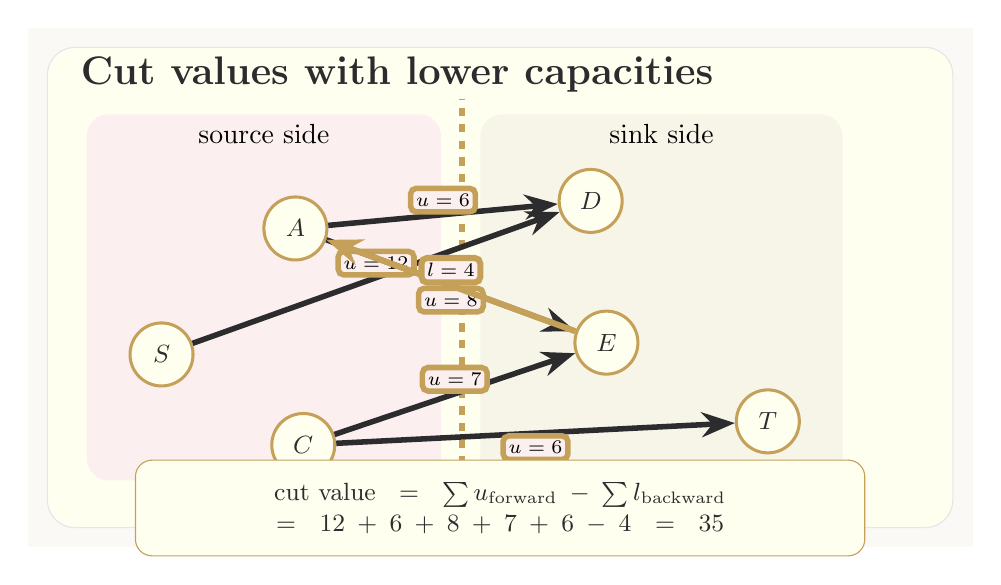
\begin{tikzpicture}[>=Stealth,vertex/.style={circle,draw=Gold,line width=1.1pt,fill=Panel,text=Ink,font=\bfseries\small,minimum size=8mm},forward/.style={->,line width=2pt,draw=Ink},backward/.style={->,line width=2.2pt,draw=Gold},fcap/.style={fill=SoftRose,draw=Gold,rounded corners=2pt,inner sep=2pt,font=\scriptsize\bfseries},formula/.style={fill=Panel,draw=Gold,rounded corners=6pt,align=center,inner sep=8pt,text=Ink,font=\small}]
\fill[Canvas] (-1.1,-2.25) rectangle (10.9,4.35);\draw[LineSoft,fill=Panel,rounded corners=10pt] (-0.85,-2.0) rectangle (10.65,4.1);\node[anchor=west,font=\bfseries\Large,text=Ink] at (-0.55,3.75){Cut values with lower capacities};
\fill[SoftRose,rounded corners=8pt] (-0.35,-1.4) rectangle (4.15,3.25);\fill[SinkTint,rounded corners=8pt] (4.65,-1.4) rectangle (9.25,3.25);\draw[Gold,line width=2.2pt,dashed] (4.42,-1.62)--(4.42,3.45);\node at (1.9,3.0){source side};\node at (6.95,3.0){sink side};
\node[vertex] (S) at (0.6,0.2) {$S$};\node[vertex] (A) at (2.3,1.8) {$A$};\node[vertex] (C) at (2.4,-0.95) {$C$};\node[vertex] (D) at (6.05,2.15) {$D$};\node[vertex] (E) at (6.25,0.35) {$E$};\node[vertex] (T) at (8.3,-0.65) {$T$};
\draw[forward] (S)--(D) node[midway,above,fcap] {$u=12$};\draw[forward] (A)--(D) node[midway,above,fcap] {$u=6$};\draw[forward] (A)--(E) node[midway,below,fcap] {$u=8$};\draw[forward] (C)--(E) node[midway,above,fcap] {$u=7$};\draw[forward] (C)--(T) node[midway,below,fcap] {$u=6$};\draw[backward] (E)--(A) node[midway,above,fcap] {$l=4$};
\node[formula,text width=8.7cm] at (4.9,-1.75){$\text{cut value}=\sum u_{\text{forward}}-\sum l_{\text{backward}}$\\$=12+6+8+7+6-4=35$};
\end{tikzpicture}\end{document}
